\documentclass[1p]{elsarticle_modified}
%\bibliographystyle{elsarticle-num}

%\usepackage[colorlinks]{hyperref}
%\usepackage{abbrmath_seonhwa} %\Abb, \Ascr, \Acal ,\Abf, \Afrak
\usepackage{amsfonts}
\usepackage{amssymb}
\usepackage{amsmath}
\usepackage{amsthm}
\usepackage{scalefnt}
\usepackage{amsbsy}
\usepackage{kotex}
\usepackage{caption}
\usepackage{subfig}
\usepackage{color}
\usepackage{graphicx}
\usepackage{xcolor} %% white, black, red, green, blue, cyan, magenta, yellow
\usepackage{float}
\usepackage{setspace}
\usepackage{hyperref}

\usepackage{tikz}
\usetikzlibrary{arrows}

\usepackage{multirow}
\usepackage{array} % fixed length table
\usepackage{hhline}

%%%%%%%%%%%%%%%%%%%%%
\makeatletter
\renewcommand*\env@matrix[1][\arraystretch]{%
	\edef\arraystretch{#1}%
	\hskip -\arraycolsep
	\let\@ifnextchar\new@ifnextchar
	\array{*\c@MaxMatrixCols c}}
\makeatother %https://tex.stackexchange.com/questions/14071/how-can-i-increase-the-line-spacing-in-a-matrix
%%%%%%%%%%%%%%%

\usepackage[normalem]{ulem}

\newcommand{\msout}[1]{\ifmmode\text{\sout{\ensuremath{#1}}}\else\sout{#1}\fi}
%SOURCE: \msout is \stkout macro in https://tex.stackexchange.com/questions/20609/strikeout-in-math-mode

\newcommand{\cancel}[1]{
	\ifmmode
	{\color{red}\msout{#1}}
	\else
	{\color{red}\sout{#1}}
	\fi
}

\newcommand{\add}[1]{
	{\color{blue}\uwave{#1}}
}

\newcommand{\replace}[2]{
	\ifmmode
	{\color{red}\msout{#1}}{\color{blue}\uwave{#2}}
	\else
	{\color{red}\sout{#1}}{\color{blue}\uwave{#2}}
	\fi
}

\newcommand{\Sol}{\mathcal{S}} %segment
\newcommand{\D}{D} %diagram
\newcommand{\A}{\mathcal{A}} %arc


%%%%%%%%%%%%%%%%%%%%%%%%%%%%%5 test

\def\sl{\operatorname{\textup{SL}}(2,\Cbb)}
\def\psl{\operatorname{\textup{PSL}}(2,\Cbb)}
\def\quan{\mkern 1mu \triangleright \mkern 1mu}

\theoremstyle{definition}
\newtheorem{thm}{Theorem}[section]
\newtheorem{prop}[thm]{Proposition}
\newtheorem{lem}[thm]{Lemma}
\newtheorem{ques}[thm]{Question}
\newtheorem{cor}[thm]{Corollary}
\newtheorem{defn}[thm]{Definition}
\newtheorem{exam}[thm]{Example}
\newtheorem{rmk}[thm]{Remark}
\newtheorem{alg}[thm]{Algorithm}

\newcommand{\I}{\sqrt{-1}}
\begin{document}

%\begin{frontmatter}
%
%\title{Boundary parabolic representations of knots up to 8 crossings}
%
%%% Group authors per affiliation:
%\author{Yunhi Cho} 
%\address{Department of Mathematics, University of Seoul, Seoul, Korea}
%\ead{yhcho@uos.ac.kr}
%
%
%\author{Seonhwa Kim} %\fnref{s_kim}}
%\address{Center for Geometry and Physics, Institute for Basic Science, Pohang, 37673, Korea}
%\ead{ryeona17@ibs.re.kr}
%
%\author{Hyuk Kim}
%\address{Department of Mathematical Sciences, Seoul National University, Seoul 08826, Korea}
%\ead{hyukkim@snu.ac.kr}
%
%\author{Seokbeom Yoon}
%\address{Department of Mathematical Sciences, Seoul National University, Seoul, 08826,  Korea}
%\ead{sbyoon15@snu.ac.kr}
%
%\begin{abstract}
%We find all boundary parabolic representation of knots up to 8 crossings.
%
%\end{abstract}
%\begin{keyword}
%    \MSC[2010] 57M25 
%\end{keyword}
%
%\end{frontmatter}

%\linenumbers
%\tableofcontents
%
\newcommand\colored[1]{\textcolor{white}{\rule[-0.35ex]{0.8em}{1.4ex}}\kern-0.8em\color{red} #1}%
%\newcommand\colored[1]{\textcolor{white}{ #1}\kern-2.17ex	\textcolor{white}{ #1}\kern-1.81ex	\textcolor{white}{ #1}\kern-2.15ex\color{red}#1	}

{\Large $\underline{11n_{98}~(K11n_{98})}$}

\setlength{\tabcolsep}{10pt}
\renewcommand{\arraystretch}{1.6}
\vspace{1cm}\begin{tabular}{m{100pt}>{\centering\arraybackslash}m{274pt}}
\multirow{5}{120pt}{
	\centering
	\includegraphics[width=112pt]{../../../GIT/diagram.site/Diagrams/png/714_11n_98.png}\\
\ \ \ A knot diagram\footnotemark}&
\allowdisplaybreaks
\textbf{Linearized knot diagam} \\
\cline{2-2}
 &
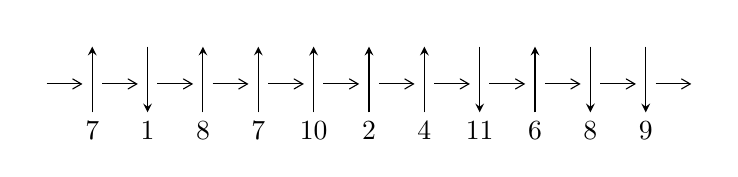
\begin{tikzpicture}[x=20pt, y=17pt]
	% nodes
	\node (C0) at (0, 0) {};
	\node (C1) at (1, 0) {};
	\node (C1U) at (1, +1) {};
	\node (C1D) at (1, -1) {7};

	\node (C2) at (2, 0) {};
	\node (C2U) at (2, +1) {};
	\node (C2D) at (2, -1) {1};

	\node (C3) at (3, 0) {};
	\node (C3U) at (3, +1) {};
	\node (C3D) at (3, -1) {8};

	\node (C4) at (4, 0) {};
	\node (C4U) at (4, +1) {};
	\node (C4D) at (4, -1) {7};

	\node (C5) at (5, 0) {};
	\node (C5U) at (5, +1) {};
	\node (C5D) at (5, -1) {10};

	\node (C6) at (6, 0) {};
	\node (C6U) at (6, +1) {};
	\node (C6D) at (6, -1) {2};

	\node (C7) at (7, 0) {};
	\node (C7U) at (7, +1) {};
	\node (C7D) at (7, -1) {4};

	\node (C8) at (8, 0) {};
	\node (C8U) at (8, +1) {};
	\node (C8D) at (8, -1) {11};

	\node (C9) at (9, 0) {};
	\node (C9U) at (9, +1) {};
	\node (C9D) at (9, -1) {6};

	\node (C10) at (10, 0) {};
	\node (C10U) at (10, +1) {};
	\node (C10D) at (10, -1) {8};

	\node (C11) at (11, 0) {};
	\node (C11U) at (11, +1) {};
	\node (C11D) at (11, -1) {9};
	\node (C12) at (12, 0) {};

	% arrows
	\draw[->,>={angle 60}]
	(C0) edge (C1) (C1) edge (C2) (C2) edge (C3) (C3) edge (C4) (C4) edge (C5) (C5) edge (C6) (C6) edge (C7) (C7) edge (C8) (C8) edge (C9) (C9) edge (C10) (C10) edge (C11) (C11) edge (C12) ;	\draw[->,>=stealth]
	(C1D) edge (C1U) (C2U) edge (C2D) (C3D) edge (C3U) (C4D) edge (C4U) (C5D) edge (C5U) (C6D) edge (C6U) (C7D) edge (C7U) (C8U) edge (C8D) (C9D) edge (C9U) (C10U) edge (C10D) (C11U) edge (C11D) ;
	\end{tikzpicture} \\
\hhline{~~} \\& 
\textbf{Solving Sequence} \\ \cline{2-2} 
 &
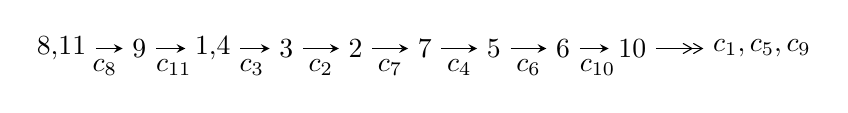
\begin{tikzpicture}[x=25pt, y=7pt]
	% node
	\node (A0) at (-1/8, 0) {8,11};
	\node (A1) at (1, 0) {9};
	\node (A2) at (33/16, 0) {1,4};
	\node (A3) at (25/8, 0) {3};
	\node (A4) at (33/8, 0) {2};
	\node (A5) at (41/8, 0) {7};
	\node (A6) at (49/8, 0) {5};
	\node (A7) at (57/8, 0) {6};
	\node (A8) at (65/8, 0) {10};
	\node (C1) at (1/2, -1) {$c_{8}$};
	\node (C2) at (3/2, -1) {$c_{11}$};
	\node (C3) at (21/8, -1) {$c_{3}$};
	\node (C4) at (29/8, -1) {$c_{2}$};
	\node (C5) at (37/8, -1) {$c_{7}$};
	\node (C6) at (45/8, -1) {$c_{4}$};
	\node (C7) at (53/8, -1) {$c_{6}$};
	\node (C8) at (61/8, -1) {$c_{10}$};
	\node (A9) at (10, 0) {$c_{1},c_{5},c_{9}$};

	% edge
	\draw[->,>=stealth]	
	(A0) edge (A1) (A1) edge (A2) (A2) edge (A3) (A3) edge (A4) (A4) edge (A5) (A5) edge (A6) (A6) edge (A7) (A7) edge (A8) ;
	\draw[->>,>={angle 60}]	
	(A8) edge (A9);
\end{tikzpicture} \\ 

\end{tabular} \\

\footnotetext{
The image of knot diagram is generated by the software ``\textbf{Draw programme}" developed by Andrew Bartholomew(\url{http://www.layer8.co.uk/maths/draw/index.htm\#Running-draw}), where we modified some parts for our purpose(\url{https://github.com/CATsTAILs/LinksPainter}).
}\phantom \\ \newline 
\centering \textbf{Ideals for irreducible components\footnotemark of $X_{\text{par}}$} 
 
\begin{align*}
I^u_{1}&=\langle 
-325810 u^{16}+546213 u^{15}+\cdots+3637114 b-2536642,\\
\phantom{I^u_{1}}&\phantom{= \langle  }-877137 u^{16}+1987958 u^{15}+\cdots+7274228 a-10784281,\;u^{17}-2 u^{16}+\cdots+13 u-4\rangle \\
I^u_{2}&=\langle 
- u^{10}+u^9+4 u^8-3 u^7-6 u^6+2 u^5+2 u^4- u^2 a+3 u^3+3 u^2+b+a-3 u-2,\;2 u^{10}-5 u^9+\cdots-4 a+5,\\
\phantom{I^u_{2}}&\phantom{= \langle  }u^{11}- u^{10}-4 u^9+3 u^8+6 u^7-2 u^6-2 u^5-3 u^4-3 u^3+3 u^2+2 u+1\rangle \\
I^u_{3}&=\langle 
a u+b+a+2 u+3,\;a^2+2 a u+4 a+2 u+6,\;u^2+u-1\rangle \\
I^u_{4}&=\langle 
b-1,\;2 a-1,\;u-1\rangle \\
\\
\end{align*}
\raggedright * 4 irreducible components of $\dim_{\mathbb{C}}=0$, with total 44 representations.\\
\footnotetext{All coefficients of polynomials are rational numbers. But the coefficients are sometimes approximated in decimal forms when there is not enough margin.}
\newpage
\renewcommand{\arraystretch}{1}
\centering \section*{I. $I^u_{1}= \langle -3.26\times10^{5} u^{16}+5.46\times10^{5} u^{15}+\cdots+3.64\times10^{6} b-2.54\times10^{6},\;-8.77\times10^{5} u^{16}+1.99\times10^{6} u^{15}+\cdots+7.27\times10^{6} a-1.08\times10^{7},\;u^{17}-2 u^{16}+\cdots+13 u-4 \rangle$}
\flushleft \textbf{(i) Arc colorings}\\
\begin{tabular}{m{7pt} m{180pt} m{7pt} m{180pt} }
\flushright $a_{8}=$&$\begin{pmatrix}1\\0\end{pmatrix}$ \\
\flushright $a_{11}=$&$\begin{pmatrix}0\\u\end{pmatrix}$ \\
\flushright $a_{9}=$&$\begin{pmatrix}1\\u^2\end{pmatrix}$ \\
\flushright $a_{1}=$&$\begin{pmatrix}- u\\- u^3+u\end{pmatrix}$ \\
\flushright $a_{4}=$&$\begin{pmatrix}0.120581 u^{16}-0.273288 u^{15}+\cdots-0.0580715 u+1.48253\\0.0895793 u^{16}-0.150178 u^{15}+\cdots+0.0542218 u+0.697433\end{pmatrix}$ \\
\flushright $a_{3}=$&$\begin{pmatrix}0.0310022 u^{16}-0.123110 u^{15}+\cdots-0.112293 u+0.785100\\0.0895793 u^{16}-0.150178 u^{15}+\cdots+0.0542218 u+0.697433\end{pmatrix}$ \\
\flushright $a_{2}=$&$\begin{pmatrix}0.239444 u^{16}-0.304221 u^{15}+\cdots-1.56094 u+1.51558\\0.205575 u^{16}-0.224465 u^{15}+\cdots-0.728410 u+0.910041\end{pmatrix}$ \\
\flushright $a_{7}=$&$\begin{pmatrix}0.235464 u^{16}-0.270574 u^{15}+\cdots-0.673677 u+2.19687\\0.182621 u^{16}-0.156800 u^{15}+\cdots-1.28067 u+0.925424\end{pmatrix}$ \\
\flushright $a_{5}=$&$\begin{pmatrix}0.360026 u^{16}-0.577509 u^{15}+\cdots-0.619016 u+2.99812\\0.295154 u^{16}-0.374642 u^{15}+\cdots-1.67419 u+1.60747\end{pmatrix}$ \\
\flushright $a_{6}=$&$\begin{pmatrix}0.474993 u^{16}-0.539864 u^{15}+\cdots-1.82912 u+3.29061\\0.410121 u^{16}-0.336997 u^{15}+\cdots-2.88429 u+1.89997\end{pmatrix}$ \\
\flushright $a_{10}=$&$\begin{pmatrix}u\\u\end{pmatrix}$\\ \flushright $a_{10}=$&$\begin{pmatrix}u\\u\end{pmatrix}$\\&\end{tabular}
\flushleft \textbf{(ii) Obstruction class $= -1$}\\~\\
\flushleft \textbf{(iii) Cusp Shapes $= \frac{9594931}{7274228} u^{16}-\frac{15193461}{7274228} u^{15}+\cdots+\frac{10670363}{7274228} u+\frac{21150807}{1818557}$}\\~\\
\newpage\renewcommand{\arraystretch}{1}
\flushleft \textbf{(iv) u-Polynomials at the component}\newline \\
\begin{tabular}{m{50pt}|m{274pt}}
Crossings & \hspace{64pt}u-Polynomials at each crossing \\
\hline $$\begin{aligned}c_{1},c_{3},c_{4}\\c_{6},c_{7}\end{aligned}$$&$\begin{aligned}
&u^{17}- u^{16}+\cdots-4 u^2-1
\end{aligned}$\\
\hline $$\begin{aligned}c_{2}\end{aligned}$$&$\begin{aligned}
&u^{17}+5 u^{16}+\cdots-8 u-1
\end{aligned}$\\
\hline $$\begin{aligned}c_{5},c_{9}\end{aligned}$$&$\begin{aligned}
&u^{17}-3 u^{16}+\cdots+22 u-8
\end{aligned}$\\
\hline $$\begin{aligned}c_{8},c_{10},c_{11}\end{aligned}$$&$\begin{aligned}
&u^{17}-2 u^{16}+\cdots+13 u-4
\end{aligned}$\\
\hline
\end{tabular}\\~\\
\newpage\renewcommand{\arraystretch}{1}
\flushleft \textbf{(v) Riley Polynomials at the component}\newline \\
\begin{tabular}{m{50pt}|m{274pt}}
Crossings & \hspace{64pt}Riley Polynomials at each crossing \\
\hline $$\begin{aligned}c_{1},c_{3},c_{4}\\c_{6},c_{7}\end{aligned}$$&$\begin{aligned}
&y^{17}+5 y^{16}+\cdots-8 y-1
\end{aligned}$\\
\hline $$\begin{aligned}c_{2}\end{aligned}$$&$\begin{aligned}
&y^{17}+13 y^{16}+\cdots-12 y-1
\end{aligned}$\\
\hline $$\begin{aligned}c_{5},c_{9}\end{aligned}$$&$\begin{aligned}
&y^{17}+9 y^{16}+\cdots-12 y-64
\end{aligned}$\\
\hline $$\begin{aligned}c_{8},c_{10},c_{11}\end{aligned}$$&$\begin{aligned}
&y^{17}-16 y^{16}+\cdots+209 y-16
\end{aligned}$\\
\hline
\end{tabular}\\~\\
\newpage\flushleft \textbf{(vi) Complex Volumes and Cusp Shapes}
$$\begin{array}{c|c|c}  
\text{Solutions to }I^u_{1}& \I (\text{vol} + \sqrt{-1}CS) & \text{Cusp shape}\\
 \hline 
\begin{aligned}
u &= -0.240053 + 0.973100 I \\
a &= \phantom{-}0.644042 - 0.652010 I \\
b &= -0.678341 - 1.093890 I\end{aligned}
 & \phantom{-}0.65577 + 8.75138 I & \phantom{-}0.84209 - 7.19652 I \\ \hline\begin{aligned}
u &= -0.240053 - 0.973100 I \\
a &= \phantom{-}0.644042 + 0.652010 I \\
b &= -0.678341 + 1.093890 I\end{aligned}
 & \phantom{-}0.65577 - 8.75138 I & \phantom{-}0.84209 + 7.19652 I \\ \hline\begin{aligned}
u &= -0.911746 + 0.271963 I \\
a &= \phantom{-}0.521420 - 0.719384 I \\
b &= -0.187558 - 0.379982 I\end{aligned}
 & -1.69658 + 0.80451 I & -2.69480 - 2.52231 I \\ \hline\begin{aligned}
u &= -0.911746 - 0.271963 I \\
a &= \phantom{-}0.521420 + 0.719384 I \\
b &= -0.187558 + 0.379982 I\end{aligned}
 & -1.69658 - 0.80451 I & -2.69480 + 2.52231 I \\ \hline\begin{aligned}
u &= \phantom{-}1.114510 + 0.218797 I \\
a &= \phantom{-}0.635665 + 0.251760 I \\
b &= \phantom{-}1.157790 + 0.487195 I\end{aligned}
 & \phantom{-}0.354258 - 0.834124 I & \phantom{-}0.06498 + 5.84789 I \\ \hline\begin{aligned}
u &= \phantom{-}1.114510 - 0.218797 I \\
a &= \phantom{-}0.635665 - 0.251760 I \\
b &= \phantom{-}1.157790 - 0.487195 I\end{aligned}
 & \phantom{-}0.354258 + 0.834124 I & \phantom{-}0.06498 - 5.84789 I \\ \hline\begin{aligned}
u &= -1.030910 + 0.649737 I \\
a &= -0.466920 + 0.601803 I \\
b &= -0.583285 + 0.914805 I\end{aligned}
 & -1.75655 - 3.15519 I & -1.08772 + 4.41422 I \\ \hline\begin{aligned}
u &= -1.030910 - 0.649737 I \\
a &= -0.466920 - 0.601803 I \\
b &= -0.583285 - 0.914805 I\end{aligned}
 & -1.75655 + 3.15519 I & -1.08772 - 4.41422 I \\ \hline\begin{aligned}
u &= \phantom{-}0.248382 + 0.709434 I \\
a &= -0.785996 - 0.998686 I \\
b &= \phantom{-}0.784905 - 0.787523 I\end{aligned}
 & \phantom{-}2.78581 - 2.60100 I & \phantom{-}4.98680 + 3.49505 I \\ \hline\begin{aligned}
u &= \phantom{-}0.248382 - 0.709434 I \\
a &= -0.785996 + 0.998686 I \\
b &= \phantom{-}0.784905 + 0.787523 I\end{aligned}
 & \phantom{-}2.78581 + 2.60100 I & \phantom{-}4.98680 - 3.49505 I\\
 \hline 
 \end{array}$$\newpage$$\begin{array}{c|c|c}  
\text{Solutions to }I^u_{1}& \I (\text{vol} + \sqrt{-1}CS) & \text{Cusp shape}\\
 \hline 
\begin{aligned}
u &= -1.44333 + 0.29962 I \\
a &= -0.27964 + 2.02194 I \\
b &= \phantom{-}0.606656 + 1.025000 I\end{aligned}
 & -2.68580 + 6.31167 I & -1.34813 - 5.64607 I \\ \hline\begin{aligned}
u &= -1.44333 - 0.29962 I \\
a &= -0.27964 - 2.02194 I \\
b &= \phantom{-}0.606656 - 1.025000 I\end{aligned}
 & -2.68580 - 6.31167 I & -1.34813 + 5.64607 I \\ \hline\begin{aligned}
u &= \phantom{-}1.43553 + 0.42213 I \\
a &= \phantom{-}0.59170 + 1.89308 I \\
b &= -0.678472 + 1.240020 I\end{aligned}
 & -4.6382 - 13.7590 I & -2.60534 + 8.09148 I \\ \hline\begin{aligned}
u &= \phantom{-}1.43553 - 0.42213 I \\
a &= \phantom{-}0.59170 - 1.89308 I \\
b &= -0.678472 - 1.240020 I\end{aligned}
 & -4.6382 + 13.7590 I & -2.60534 - 8.09148 I \\ \hline\begin{aligned}
u &= \phantom{-}1.67968 + 0.04846 I \\
a &= -0.20221 - 1.49330 I \\
b &= -0.239314 - 0.869369 I\end{aligned}
 & -11.59490 + 1.04318 I & -1.35194 - 7.04363 I \\ \hline\begin{aligned}
u &= \phantom{-}1.67968 - 0.04846 I \\
a &= -0.20221 + 1.49330 I \\
b &= -0.239314 + 0.869369 I\end{aligned}
 & -11.59490 - 1.04318 I & -1.35194 + 7.04363 I \\ \hline\begin{aligned}
u &= \phantom{-}0.295856\phantom{ +0.000000I} \\
a &= \phantom{-}1.43389\phantom{ +0.000000I} \\
b &= \phantom{-}0.635251\phantom{ +0.000000I}\end{aligned}
 & \phantom{-}0.963952\phantom{ +0.000000I} & \phantom{-}10.6380\phantom{ +0.000000I}\\
 \hline 
 \end{array}$$\newpage\newpage\renewcommand{\arraystretch}{1}
\centering \section*{II. $I^u_{2}= \langle - u^{10}+u^9+\cdots+a-2,\;2 u^{10}-5 u^9+\cdots-4 a+5,\;u^{11}- u^{10}+\cdots+2 u+1 \rangle$}
\flushleft \textbf{(i) Arc colorings}\\
\begin{tabular}{m{7pt} m{180pt} m{7pt} m{180pt} }
\flushright $a_{8}=$&$\begin{pmatrix}1\\0\end{pmatrix}$ \\
\flushright $a_{11}=$&$\begin{pmatrix}0\\u\end{pmatrix}$ \\
\flushright $a_{9}=$&$\begin{pmatrix}1\\u^2\end{pmatrix}$ \\
\flushright $a_{1}=$&$\begin{pmatrix}- u\\- u^3+u\end{pmatrix}$ \\
\flushright $a_{4}=$&$\begin{pmatrix}a\\u^{10}- u^9-4 u^8+3 u^7+6 u^6-2 u^5-2 u^4+u^2 a-3 u^3-3 u^2- a+3 u+2\end{pmatrix}$ \\
\flushright $a_{3}=$&$\begin{pmatrix}- u^{10}+u^9+\cdots+2 a-2\\u^{10}- u^9-4 u^8+3 u^7+6 u^6-2 u^5-2 u^4+u^2 a-3 u^3-3 u^2- a+3 u+2\end{pmatrix}$ \\
\flushright $a_{2}=$&$\begin{pmatrix}- u^{10}+u^9+\cdots+2 a-2\\u^{10}- u^9+\cdots- a+2\end{pmatrix}$ \\
\flushright $a_{7}=$&$\begin{pmatrix}- u^{10} a+2 u^{10}+\cdots-2 a+3\\- u^5 a- u^6+2 u^3 a+2 u^4- a u-2\end{pmatrix}$ \\
\flushright $a_{5}=$&$\begin{pmatrix}u^7-2 u^5+2 u\\u^9-3 u^7+3 u^5- u\end{pmatrix}$ \\
\flushright $a_{6}=$&$\begin{pmatrix}u^{10}-3 u^8+2 u^6+3 u^4-3 u^2-1\\u^{10}+u^9-3 u^8-4 u^7+2 u^6+5 u^5+3 u^4-3 u^2-3 u-1\end{pmatrix}$ \\
\flushright $a_{10}=$&$\begin{pmatrix}u\\u\end{pmatrix}$\\ \flushright $a_{10}=$&$\begin{pmatrix}u\\u\end{pmatrix}$\\&\end{tabular}
\flushleft \textbf{(ii) Obstruction class $= -1$}\\~\\
\flushleft \textbf{(iii) Cusp Shapes $= 4 u^9-16 u^7-4 u^6+20 u^5+12 u^4+4 u^3-8 u^2-20 u-6$}\\~\\
\newpage\renewcommand{\arraystretch}{1}
\flushleft \textbf{(iv) u-Polynomials at the component}\newline \\
\begin{tabular}{m{50pt}|m{274pt}}
Crossings & \hspace{64pt}u-Polynomials at each crossing \\
\hline $$\begin{aligned}c_{1},c_{3},c_{4}\\c_{6},c_{7}\end{aligned}$$&$\begin{aligned}
&u^{22}+3 u^{21}+\cdots+24 u+9
\end{aligned}$\\
\hline $$\begin{aligned}c_{2}\end{aligned}$$&$\begin{aligned}
&u^{22}+11 u^{21}+\cdots+432 u+81
\end{aligned}$\\
\hline $$\begin{aligned}c_{5},c_{9}\end{aligned}$$&$\begin{aligned}
&(u^{11}+u^{10}+2 u^9+u^8+4 u^7+2 u^6+4 u^5+u^4+3 u^3- u^2-1)^2
\end{aligned}$\\
\hline $$\begin{aligned}c_{8},c_{10},c_{11}\end{aligned}$$&$\begin{aligned}
&(u^{11}- u^{10}-4 u^9+3 u^8+6 u^7-2 u^6-2 u^5-3 u^4-3 u^3+3 u^2+2 u+1)^2
\end{aligned}$\\
\hline
\end{tabular}\\~\\
\newpage\renewcommand{\arraystretch}{1}
\flushleft \textbf{(v) Riley Polynomials at the component}\newline \\
\begin{tabular}{m{50pt}|m{274pt}}
Crossings & \hspace{64pt}Riley Polynomials at each crossing \\
\hline $$\begin{aligned}c_{1},c_{3},c_{4}\\c_{6},c_{7}\end{aligned}$$&$\begin{aligned}
&y^{22}+11 y^{21}+\cdots+432 y+81
\end{aligned}$\\
\hline $$\begin{aligned}c_{2}\end{aligned}$$&$\begin{aligned}
&y^{22}- y^{21}+\cdots+35640 y+6561
\end{aligned}$\\
\hline $$\begin{aligned}c_{5},c_{9}\end{aligned}$$&$\begin{aligned}
&(y^{11}+3 y^{10}+\cdots-2 y-1)^{2}
\end{aligned}$\\
\hline $$\begin{aligned}c_{8},c_{10},c_{11}\end{aligned}$$&$\begin{aligned}
&(y^{11}-9 y^{10}+\cdots-2 y-1)^{2}
\end{aligned}$\\
\hline
\end{tabular}\\~\\
\newpage\flushleft \textbf{(vi) Complex Volumes and Cusp Shapes}
$$\begin{array}{c|c|c}  
\text{Solutions to }I^u_{2}& \I (\text{vol} + \sqrt{-1}CS) & \text{Cusp shape}\\
 \hline 
\begin{aligned}
u &= -1.14725\phantom{ +0.000000I} \\
a &= -2.18308 + 3.31504 I \\
b &= \phantom{-}0.181376 + 1.048190 I\end{aligned}
 & -5.48524\phantom{ +0.000000I} & \phantom{-}0.376260\phantom{ +0.000000I} \\ \hline\begin{aligned}
u &= -1.14725\phantom{ +0.000000I} \\
a &= -2.18308 - 3.31504 I \\
b &= \phantom{-}0.181376 - 1.048190 I\end{aligned}
 & -5.48524\phantom{ +0.000000I} & \phantom{-}0.376260\phantom{ +0.000000I} \\ \hline\begin{aligned}
u &= -0.044199 + 0.849205 I \\
a &= \phantom{-}0.547434 + 0.348829 I \\
b &= -0.853835 + 0.533591 I\end{aligned}
 & \phantom{-}2.35273 + 3.04152 I & \phantom{-}4.06121 - 2.82242 I \\ \hline\begin{aligned}
u &= -0.044199 + 0.849205 I \\
a &= -0.372720 + 0.162477 I \\
b &= \phantom{-}0.714099 + 0.923041 I\end{aligned}
 & \phantom{-}2.35273 + 3.04152 I & \phantom{-}4.06121 - 2.82242 I \\ \hline\begin{aligned}
u &= -0.044199 - 0.849205 I \\
a &= \phantom{-}0.547434 - 0.348829 I \\
b &= -0.853835 - 0.533591 I\end{aligned}
 & \phantom{-}2.35273 - 3.04152 I & \phantom{-}4.06121 + 2.82242 I \\ \hline\begin{aligned}
u &= -0.044199 - 0.849205 I \\
a &= -0.372720 - 0.162477 I \\
b &= \phantom{-}0.714099 - 0.923041 I\end{aligned}
 & \phantom{-}2.35273 - 3.04152 I & \phantom{-}4.06121 + 2.82242 I \\ \hline\begin{aligned}
u &= -1.232090 + 0.392876 I \\
a &= \phantom{-}0.674566 - 0.370203 I \\
b &= \phantom{-}0.623653 - 0.552777 I\end{aligned}
 & -1.31282 + 1.41699 I & \phantom{-}0.791306 - 0.633731 I \\ \hline\begin{aligned}
u &= -1.232090 + 0.392876 I \\
a &= \phantom{-}0.48177 - 1.51619 I \\
b &= -0.555909 - 0.782909 I\end{aligned}
 & -1.31282 + 1.41699 I & \phantom{-}0.791306 - 0.633731 I \\ \hline\begin{aligned}
u &= -1.232090 - 0.392876 I \\
a &= \phantom{-}0.674566 + 0.370203 I \\
b &= \phantom{-}0.623653 + 0.552777 I\end{aligned}
 & -1.31282 - 1.41699 I & \phantom{-}0.791306 + 0.633731 I \\ \hline\begin{aligned}
u &= -1.232090 - 0.392876 I \\
a &= \phantom{-}0.48177 + 1.51619 I \\
b &= -0.555909 + 0.782909 I\end{aligned}
 & -1.31282 - 1.41699 I & \phantom{-}0.791306 + 0.633731 I\\
 \hline 
 \end{array}$$\newpage$$\begin{array}{c|c|c}  
\text{Solutions to }I^u_{2}& \I (\text{vol} + \sqrt{-1}CS) & \text{Cusp shape}\\
 \hline 
\begin{aligned}
u &= \phantom{-}1.317220 + 0.129556 I \\
a &= \phantom{-}0.469425 + 0.990105 I \\
b &= -0.752651 + 0.945347 I\end{aligned}
 & -8.47148 - 2.94672 I & -5.79937 + 4.11787 I \\ \hline\begin{aligned}
u &= \phantom{-}1.317220 + 0.129556 I \\
a &= -0.15850 - 2.09923 I \\
b &= -0.14927 - 1.48798 I\end{aligned}
 & -8.47148 - 2.94672 I & -5.79937 + 4.11787 I \\ \hline\begin{aligned}
u &= \phantom{-}1.317220 - 0.129556 I \\
a &= \phantom{-}0.469425 - 0.990105 I \\
b &= -0.752651 - 0.945347 I\end{aligned}
 & -8.47148 + 2.94672 I & -5.79937 - 4.11787 I \\ \hline\begin{aligned}
u &= \phantom{-}1.317220 - 0.129556 I \\
a &= -0.15850 + 2.09923 I \\
b &= -0.14927 + 1.48798 I\end{aligned}
 & -8.47148 + 2.94672 I & -5.79937 - 4.11787 I \\ \hline\begin{aligned}
u &= \phantom{-}1.304640 + 0.385413 I \\
a &= -0.579828 + 0.055525 I \\
b &= -1.081770 - 0.344108 I\end{aligned}
 & -1.85809 - 7.47524 I & -0.22908 + 5.55460 I \\ \hline\begin{aligned}
u &= \phantom{-}1.304640 + 0.385413 I \\
a &= -0.45041 - 1.69192 I \\
b &= \phantom{-}0.747184 - 1.181250 I\end{aligned}
 & -1.85809 - 7.47524 I & -0.22908 + 5.55460 I \\ \hline\begin{aligned}
u &= \phantom{-}1.304640 - 0.385413 I \\
a &= -0.579828 - 0.055525 I \\
b &= -1.081770 + 0.344108 I\end{aligned}
 & -1.85809 + 7.47524 I & -0.22908 - 5.55460 I \\ \hline\begin{aligned}
u &= \phantom{-}1.304640 - 0.385413 I \\
a &= -0.45041 + 1.69192 I \\
b &= \phantom{-}0.747184 + 1.181250 I\end{aligned}
 & -1.85809 + 7.47524 I & -0.22908 - 5.55460 I \\ \hline\begin{aligned}
u &= -0.271947 + 0.385187 I \\
a &= \phantom{-}1.270550 + 0.259399 I \\
b &= -0.087548 + 1.187670 I\end{aligned}
 & -3.59460 + 1.13130 I & -0.01220 - 6.05785 I \\ \hline\begin{aligned}
u &= -0.271947 + 0.385187 I \\
a &= \phantom{-}1.80079 + 2.03466 I \\
b &= -0.285332 - 0.830788 I\end{aligned}
 & -3.59460 + 1.13130 I & -0.01220 - 6.05785 I\\
 \hline 
 \end{array}$$\newpage$$\begin{array}{c|c|c}  
\text{Solutions to }I^u_{2}& \I (\text{vol} + \sqrt{-1}CS) & \text{Cusp shape}\\
 \hline 
\begin{aligned}
u &= -0.271947 - 0.385187 I \\
a &= \phantom{-}1.270550 - 0.259399 I \\
b &= -0.087548 - 1.187670 I\end{aligned}
 & -3.59460 - 1.13130 I & -0.01220 + 6.05785 I \\ \hline\begin{aligned}
u &= -0.271947 - 0.385187 I \\
a &= \phantom{-}1.80079 - 2.03466 I \\
b &= -0.285332 + 0.830788 I\end{aligned}
 & -3.59460 - 1.13130 I & -0.01220 + 6.05785 I\\
 \hline 
 \end{array}$$\newpage\newpage\renewcommand{\arraystretch}{1}
\centering \section*{III. $I^u_{3}= \langle a u+b+a+2 u+3,\;a^2+2 a u+4 a+2 u+6,\;u^2+u-1 \rangle$}
\flushleft \textbf{(i) Arc colorings}\\
\begin{tabular}{m{7pt} m{180pt} m{7pt} m{180pt} }
\flushright $a_{8}=$&$\begin{pmatrix}1\\0\end{pmatrix}$ \\
\flushright $a_{11}=$&$\begin{pmatrix}0\\u\end{pmatrix}$ \\
\flushright $a_{9}=$&$\begin{pmatrix}1\\- u+1\end{pmatrix}$ \\
\flushright $a_{1}=$&$\begin{pmatrix}- u\\- u+1\end{pmatrix}$ \\
\flushright $a_{4}=$&$\begin{pmatrix}a\\- a u- a-2 u-3\end{pmatrix}$ \\
\flushright $a_{3}=$&$\begin{pmatrix}a u+2 a+2 u+3\\- a u- a-2 u-3\end{pmatrix}$ \\
\flushright $a_{2}=$&$\begin{pmatrix}a u+2 a+u+3\\- a u- a-3 u-2\end{pmatrix}$ \\
\flushright $a_{7}=$&$\begin{pmatrix}2 a u+3 a+6 u+9\\-1\end{pmatrix}$ \\
\flushright $a_{5}=$&$\begin{pmatrix}- a u- a-2 u-3\\0\end{pmatrix}$ \\
\flushright $a_{6}=$&$\begin{pmatrix}- a- u-2\\a u+u+1\end{pmatrix}$ \\
\flushright $a_{10}=$&$\begin{pmatrix}u\\u\end{pmatrix}$\\ \flushright $a_{10}=$&$\begin{pmatrix}u\\u\end{pmatrix}$\\&\end{tabular}
\flushleft \textbf{(ii) Obstruction class $= 1$}\\~\\
\flushleft \textbf{(iii) Cusp Shapes $= -8$}\\~\\
\newpage\renewcommand{\arraystretch}{1}
\flushleft \textbf{(iv) u-Polynomials at the component}\newline \\
\begin{tabular}{m{50pt}|m{274pt}}
Crossings & \hspace{64pt}u-Polynomials at each crossing \\
\hline $$\begin{aligned}c_{1},c_{3},c_{4}\\c_{6},c_{7}\end{aligned}$$&$\begin{aligned}
&(u^2+1)^2
\end{aligned}$\\
\hline $$\begin{aligned}c_{2}\end{aligned}$$&$\begin{aligned}
&(u+1)^4
\end{aligned}$\\
\hline $$\begin{aligned}c_{5},c_{9}\end{aligned}$$&$\begin{aligned}
&u^4+3 u^2+1
\end{aligned}$\\
\hline $$\begin{aligned}c_{8}\end{aligned}$$&$\begin{aligned}
&(u^2+u-1)^2
\end{aligned}$\\
\hline $$\begin{aligned}c_{10},c_{11}\end{aligned}$$&$\begin{aligned}
&(u^2- u-1)^2
\end{aligned}$\\
\hline
\end{tabular}\\~\\
\newpage\renewcommand{\arraystretch}{1}
\flushleft \textbf{(v) Riley Polynomials at the component}\newline \\
\begin{tabular}{m{50pt}|m{274pt}}
Crossings & \hspace{64pt}Riley Polynomials at each crossing \\
\hline $$\begin{aligned}c_{1},c_{3},c_{4}\\c_{6},c_{7}\end{aligned}$$&$\begin{aligned}
&(y+1)^4
\end{aligned}$\\
\hline $$\begin{aligned}c_{2}\end{aligned}$$&$\begin{aligned}
&(y-1)^4
\end{aligned}$\\
\hline $$\begin{aligned}c_{5},c_{9}\end{aligned}$$&$\begin{aligned}
&(y^2+3 y+1)^2
\end{aligned}$\\
\hline $$\begin{aligned}c_{8},c_{10},c_{11}\end{aligned}$$&$\begin{aligned}
&(y^2-3 y+1)^2
\end{aligned}$\\
\hline
\end{tabular}\\~\\
\newpage\flushleft \textbf{(vi) Complex Volumes and Cusp Shapes}
$$\begin{array}{c|c|c}  
\text{Solutions to }I^u_{3}& \I (\text{vol} + \sqrt{-1}CS) & \text{Cusp shape}\\
 \hline 
\begin{aligned}
u &= \phantom{-}0.618034\phantom{ +0.000000I} \\
a &= -2.61803 + 0.61803 I \\
b &= \phantom{-0.000000 } -1.000000 I\end{aligned}
 & -4.27683\phantom{ +0.000000I} & -8.00000\phantom{ +0.000000I} \\ \hline\begin{aligned}
u &= \phantom{-}0.618034\phantom{ +0.000000I} \\
a &= -2.61803 - 0.61803 I \\
b &= \phantom{-0.000000 -}1.000000 I\end{aligned}
 & -4.27683\phantom{ +0.000000I} & -8.00000\phantom{ +0.000000I} \\ \hline\begin{aligned}
u &= -1.61803\phantom{ +0.000000I} \\
a &= -0.38197 + 1.61803 I \\
b &= \phantom{-0.000000 -}1.000000 I\end{aligned}
 & -12.1725\phantom{ +0.000000I} & -8.00000\phantom{ +0.000000I} \\ \hline\begin{aligned}
u &= -1.61803\phantom{ +0.000000I} \\
a &= -0.38197 - 1.61803 I \\
b &= \phantom{-0.000000 } -1.000000 I\end{aligned}
 & -12.1725\phantom{ +0.000000I} & -8.00000\phantom{ +0.000000I}\\
 \hline 
 \end{array}$$\newpage\newpage\renewcommand{\arraystretch}{1}
\centering \section*{IV. $I^u_{4}= \langle b-1,\;2 a-1,\;u-1 \rangle$}
\flushleft \textbf{(i) Arc colorings}\\
\begin{tabular}{m{7pt} m{180pt} m{7pt} m{180pt} }
\flushright $a_{8}=$&$\begin{pmatrix}1\\0\end{pmatrix}$ \\
\flushright $a_{11}=$&$\begin{pmatrix}0\\1\end{pmatrix}$ \\
\flushright $a_{9}=$&$\begin{pmatrix}1\\1\end{pmatrix}$ \\
\flushright $a_{1}=$&$\begin{pmatrix}-1\\0\end{pmatrix}$ \\
\flushright $a_{4}=$&$\begin{pmatrix}0.5\\1\end{pmatrix}$ \\
\flushright $a_{3}=$&$\begin{pmatrix}-0.5\\1\end{pmatrix}$ \\
\flushright $a_{2}=$&$\begin{pmatrix}0.5\\1\end{pmatrix}$ \\
\flushright $a_{7}=$&$\begin{pmatrix}1.5\\1\end{pmatrix}$ \\
\flushright $a_{5}=$&$\begin{pmatrix}2\\2\end{pmatrix}$ \\
\flushright $a_{6}=$&$\begin{pmatrix}2\\2\end{pmatrix}$ \\
\flushright $a_{10}=$&$\begin{pmatrix}1\\1\end{pmatrix}$\\ \flushright $a_{10}=$&$\begin{pmatrix}1\\1\end{pmatrix}$\\&\end{tabular}
\flushleft \textbf{(ii) Obstruction class $= 1$}\\~\\
\flushleft \textbf{(iii) Cusp Shapes $= -2.25$}\\~\\
\newpage\renewcommand{\arraystretch}{1}
\flushleft \textbf{(iv) u-Polynomials at the component}\newline \\
\begin{tabular}{m{50pt}|m{274pt}}
Crossings & \hspace{64pt}u-Polynomials at each crossing \\
\hline $$\begin{aligned}c_{1},c_{3},c_{4}\\c_{10},c_{11}\end{aligned}$$&$\begin{aligned}
&u+1
\end{aligned}$\\
\hline $$\begin{aligned}c_{2},c_{6},c_{7}\\c_{8}\end{aligned}$$&$\begin{aligned}
&u-1
\end{aligned}$\\
\hline $$\begin{aligned}c_{5},c_{9}\end{aligned}$$&$\begin{aligned}
&u
\end{aligned}$\\
\hline
\end{tabular}\\~\\
\newpage\renewcommand{\arraystretch}{1}
\flushleft \textbf{(v) Riley Polynomials at the component}\newline \\
\begin{tabular}{m{50pt}|m{274pt}}
Crossings & \hspace{64pt}Riley Polynomials at each crossing \\
\hline $$\begin{aligned}c_{1},c_{2},c_{3}\\c_{4},c_{6},c_{7}\\c_{8},c_{10},c_{11}\end{aligned}$$&$\begin{aligned}
&y-1
\end{aligned}$\\
\hline $$\begin{aligned}c_{5},c_{9}\end{aligned}$$&$\begin{aligned}
&y
\end{aligned}$\\
\hline
\end{tabular}\\~\\
\newpage\flushleft \textbf{(vi) Complex Volumes and Cusp Shapes}
$$\begin{array}{c|c|c}  
\text{Solutions to }I^u_{4}& \I (\text{vol} + \sqrt{-1}CS) & \text{Cusp shape}\\
 \hline 
\begin{aligned}
u &= \phantom{-}1.00000\phantom{ +0.000000I} \\
a &= \phantom{-}0.500000\phantom{ +0.000000I} \\
b &= \phantom{-}1.00000\phantom{ +0.000000I}\end{aligned}
 & \phantom{-0.000000 } 0 & -2.25000\phantom{ +0.000000I}\\
 \hline 
 \end{array}$$\newpage
\newpage\renewcommand{\arraystretch}{1}
\centering \section*{ V. u-Polynomials}
\begin{tabular}{m{50pt}|m{274pt}}
Crossings & \hspace{64pt}u-Polynomials at each crossing \\
\hline $$\begin{aligned}c_{1},c_{3},c_{4}\end{aligned}$$&$\begin{aligned}
&(u+1)(u^2+1)^2(u^{17}-u^{16}+\cdots-4 u^{2}-1)(u^{22}+3 u^{21}+\cdots+24 u+9)
\end{aligned}$\\
\hline $$\begin{aligned}c_{2}\end{aligned}$$&$\begin{aligned}
&(u-1)(u+1)^4(u^{17}+5 u^{16}+\cdots-8 u-1)\\
&\cdot(u^{22}+11 u^{21}+\cdots+432 u+81)
\end{aligned}$\\
\hline $$\begin{aligned}c_{5},c_{9}\end{aligned}$$&$\begin{aligned}
&u(u^4+3 u^2+1)\\
&\cdot(u^{11}+u^{10}+2 u^9+u^8+4 u^7+2 u^6+4 u^5+u^4+3 u^3- u^2-1)^2\\
&\cdot(u^{17}-3 u^{16}+\cdots+22 u-8)
\end{aligned}$\\
\hline $$\begin{aligned}c_{6},c_{7}\end{aligned}$$&$\begin{aligned}
&(u-1)(u^2+1)^2(u^{17}-u^{16}+\cdots-4 u^{2}-1)(u^{22}+3 u^{21}+\cdots+24 u+9)
\end{aligned}$\\
\hline $$\begin{aligned}c_{8}\end{aligned}$$&$\begin{aligned}
&(u-1)(u^2+u-1)^2\\
&\cdot(u^{11}- u^{10}-4 u^9+3 u^8+6 u^7-2 u^6-2 u^5-3 u^4-3 u^3+3 u^2+2 u+1)^2\\
&\cdot(u^{17}-2 u^{16}+\cdots+13 u-4)
\end{aligned}$\\
\hline $$\begin{aligned}c_{10},c_{11}\end{aligned}$$&$\begin{aligned}
&(u+1)(u^2- u-1)^2\\
&\cdot(u^{11}- u^{10}-4 u^9+3 u^8+6 u^7-2 u^6-2 u^5-3 u^4-3 u^3+3 u^2+2 u+1)^2\\
&\cdot(u^{17}-2 u^{16}+\cdots+13 u-4)
\end{aligned}$\\
\hline
\end{tabular}\newpage\renewcommand{\arraystretch}{1}
\centering \section*{ VI. Riley Polynomials}
\begin{tabular}{m{50pt}|m{274pt}}
Crossings & \hspace{64pt}Riley Polynomials at each crossing \\
\hline $$\begin{aligned}c_{1},c_{3},c_{4}\\c_{6},c_{7}\end{aligned}$$&$\begin{aligned}
&(y-1)(y+1)^4(y^{17}+5 y^{16}+\cdots-8 y-1)\\
&\cdot(y^{22}+11 y^{21}+\cdots+432 y+81)
\end{aligned}$\\
\hline $$\begin{aligned}c_{2}\end{aligned}$$&$\begin{aligned}
&((y-1)^5)(y^{17}+13 y^{16}+\cdots-12 y-1)\\
&\cdot(y^{22}- y^{21}+\cdots+35640 y+6561)
\end{aligned}$\\
\hline $$\begin{aligned}c_{5},c_{9}\end{aligned}$$&$\begin{aligned}
&y(y^2+3 y+1)^2(y^{11}+3 y^{10}+\cdots-2 y-1)^{2}\\
&\cdot(y^{17}+9 y^{16}+\cdots-12 y-64)
\end{aligned}$\\
\hline $$\begin{aligned}c_{8},c_{10},c_{11}\end{aligned}$$&$\begin{aligned}
&(y-1)(y^2-3 y+1)^2(y^{11}-9 y^{10}+\cdots-2 y-1)^{2}\\
&\cdot(y^{17}-16 y^{16}+\cdots+209 y-16)
\end{aligned}$\\
\hline
\end{tabular}
\vskip 2pc
\end{document}